\chapter{Theory}
\label{chap:Theory}
%Escribir resumen sobre los métodos de clasificación y minería de datos

\section{Clustering}
Clustering is defined as the process of classifying a large group of data items into smaller groups that share the same or similar properties.
A cluster is a basic unit of classification of initial unclassified data based on common properties.  There are various definitions of a cluster as follows:
\begin{itemize}
\item[*] A cluster is a set of entities that are alike or a set of entities from different clusters that are not alike.
\item[*] A cluster is an aggregation of points in the test space such that the distance between any two points in the cluster is less than the distance between any point within the cluster and any other point outside the cluster.
\item[*] A cluster is a connected region of a multidimensional space containing a relatively high density of points.
\item[*] A cluster is a group of contiguous elements of a statistical population.
\end{itemize}
From these definitions, we can see that whether clusters consist of entities, points, or regions, the components within a cluster are more similar in some respects to each other than to other components outside of the cluster or to entities classified into other clusters.
This description covers two important points. One is similar, which can be reflected with distance measures, and the other is classification, which suggests the objective of clustering.
Therefore, clustering can be defined as a process of identifying groups of data that are similar in a certain aspect and building a classification among them.
A clustering process usually involves the following steps:
\begin{itemize}
\item[*]\textbf{Object Selection:} The entities to be clustered are selected in a manner such that the entities are representations of the cluster structures that are inherent in the data.
\item[*]\textbf{Variable Selection:} The variable that will represent the measurements of the entities must be selected.  Correct selection of the variable will result in a meaningful cluster structure
\item[*]\textbf{Variable Standardization:} Since variables may be measured with different systems, they may initially be incomparable.  To solve this problem, the variables are usually standardized, although this step is optional.
\item[*]\textbf{Similarity Measurement:} Similarity or dissimilarity between a pair of data items or among many items must be calculated.  This will usually be the basis of a similarity matrix.  Sometimes more than one attribute can be considered and analyzed.  This is called multivariate analysis.
\item[*]\textbf{Clustering Entities:} Based on the similarity or dissimilarity measurement a pair of items can be compared and classified in the same group or different groups.  This process is applied to all items in one data record until the items can be classified into two clusters.  Recursively following this step will result in a classification with various clusters.
\end{itemize}
\subsection{\textit{Distance Measures}}
The most commonly used proximity measure, is the Minkowsky metric, which is a generalization of the normal distance between points in the Euclidian space.  It is defined as
$$p_{ij}=\left(\sum_{k=1}^{d}\vert x_{ik}-x_{jk}\vert^{r}\right)^{1/r}$$
where $r$ is a parameter, $d$ is the dimensionality of the data object, and $x_{ik}$ and $x_{jk}$ are, respectively, the $k^{th}$ components of the $i^{th}$ and $j^{th}$ objects, $x_{i}$ and $x_{j}$.
The following is a list of the common Minkowski distances for specific values of $r$.
\begin{itemize}
\item[1.] $r=1$. City block (Manhattan, taxicap, $L_{1}$ norm) distance.  A common example of this is the Hamming distance, which is just the number of bits that are different between two binary vectors.
\item[2.] $r=2$. Euclidean distance.  The most common measure of the distance between two points.
\item[3.] $r=\infty$. ``supremum'' ($L_{max}$ norm, $L_{\infty}$ norm) distance.  This is the maximum difference between any component of the vectors.
\end{itemize}
\section{K-means}
The \textit{K-means} algorithm takes the input parameter, $k$, and partitions a set of $n$ objects into $k$ clusters so that the resulting intracluster similarity is high but the intercluster similarity is low.  Cluster similarity measures in regard to the mean value of the objects in a cluster, which can be viewed as the cluster centroid or center of gravity.
The \textit{k-means} algorithm proceeds as follows.  First, it randomly selects $k$ of the objects, each of which initially represents a cluster mean or center.  For each of the remaining objects, an object is assigned to the cluster to which it is the most similar, based on the distance between the object and the cluster mean.  It then computes the new mean for each cluster.  This process iterates until the criterion function converges.  Typically, the square-error criterion 	is used, defined as
$$E=\sum_{i=1}^{k}\sum_{p\in C_{i}}\vert p-m_{i}\vert^{2},$$
where $E$ is the sum of the square error for all objects in the data set; $p$ is the point in space representing a given object; and $m_{i}$ is the mean of cluster $C_{i}$ (both $p$ and $m_{i}$ are multidimensional).
In other words, for each object in each cluster, the distance from the object to its cluster center is square, and the distances are summed.
This criterion tries to make the resulting $k$ clusters, as compact and as separate as possible.
\textbf{Algorithm:} \textit{k-means}.  The \textit{k-means} algorithm for partitioning, where each cluster's center is represented by the mean value of the objects in the cluster.
\textbf{Input:}
\begin{itemize}
\item[*] $k$: the number of clusters,
\item[*] $D$: a data set containing $n$ objects.
\end{itemize}
\textbf{Output:} A set of $k$ clusters.
\textbf{Method:}
\begin{itemize}
\item[1)] arbitrarily choose $k$ objects from $D$ as the initial cluster centers;
\item[2)] repeat
\item[3)] re-assign each object to the cluster to which the object is the most similar, based on the mean value of the objects in the cluster;
\item[4)] update the cluster means, i.e., calculate the mean value of the objects for each cluster;
\item[5)] until no change.
\end{itemize}
\section{Decision Tree}
A decision tree is a flowchart-like tree structure, where each internal node denotes a test on an attribute, each branch represents an outcome of the test, an each leaf node (or terminal node) holds a class label. The topmost node in a tree is the root node.
\begin{figure}[ht!]
  \centering
  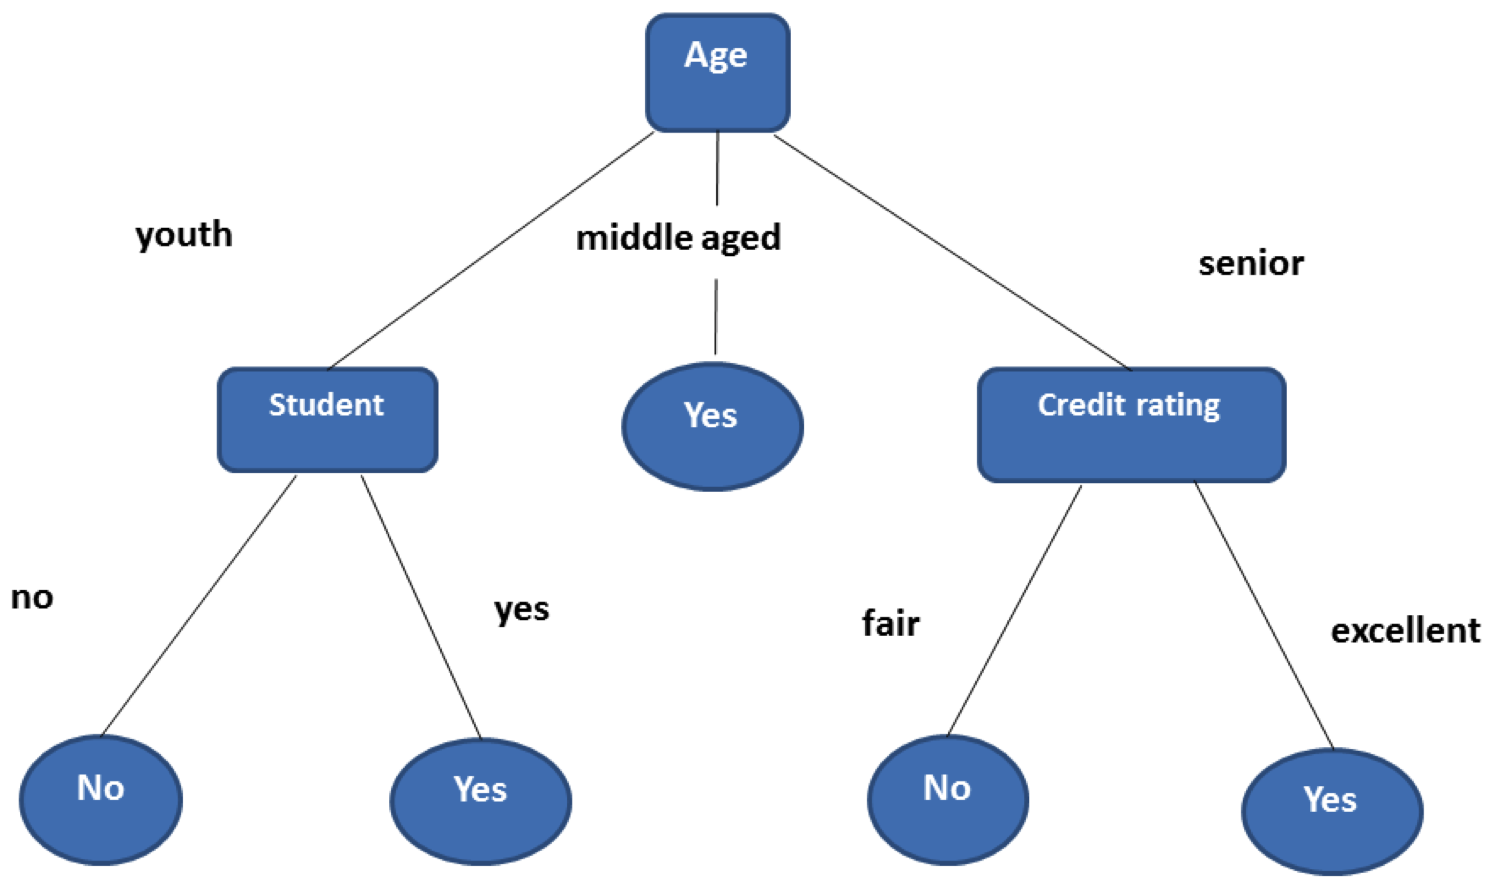
\includegraphics[scale=0.4]{arbol}
  \caption{caption}

\end{figure}
A typical decision tree is shown in Figure.  It represents the concept \textit{buys cell phone}, that is, it predicts whether a customer at AllElectronics is likely to purchase a cell phone.
Internal nodes are denoted by rectangles, and leaf nodes are denoted by ovals.  Some decision tree algorithms produce only binary trees, whereas others can produce nonbinary trees.
The construction of decision tree classifiers does not require any domain knowledge or parameter setting, and therefore is appropriate for exploratory knowledge discovery.  Decision trees can handle high dimensional data.  The learning and classification steps of decision tree induction are simple and fast.  In general, decision tree classifiers have good accuracy.
The strategy for make a decision tree is as follows:
\begin{itemize}
\item[*] The algorithm is called with three parameters: \textit{D}, \textit{attribute list}, and \textit{attribute selection method}. We refer to \textit{D}as a data partition.
The parameter \textit{attribute list} is a list of attributes describing the tuples.  \textit{attribute selection method} specifies a heuristic procedure for selecting the attribute that best discriminates the given tuples according to class.
\item[*] The tree starts as a single node, \textit{N}, representing the training tuples in \textit{D}.
\item[*] If the tuples in \textit{D} are all of the same class, then the node \textit{N} becomes a leaf and is labeled with that class.
\item[*] Otherwise, the algorithm calls \textit{attribute selection method} to determine the splitting criterion.  The splitting criterion tell us which attribute to test at node \textit{N} by determining the best way to separate or partition the tuples in \textit{D} into individual classes.  The splitting criterion is determined so that, ideally, the resulting partitions at each branch are as pure as posible.  A partition is pure if all of the tuples in it belong to the same class.
\item[*] The node \textit{N} is labeled with the splitting criterion, which serves as a test at the node. A branch is grown from node \textit{N} for each of the outcomes of the splitting criterion.  The tuples in \textit{D} are partitioned accordingly.  Let \textit{A} be the splitting attribute.  \textit{A} has $v$ distinct values, $\{a_{1}, a_ {2}, \cdots, a_{v}\}$, based on the training data.
\begin{itemize}
\item[1.] \textit{A} is \textit{discrete valued:} In this case, the outcomes of the test at node \textit{N} correspond directly to the known values of \textit{A}.  A branch is created for each known value, $a_{j}$, of \textit{A} and labeled with that value.
\item[2.] \textit{A} is \textit{continuous valued:} In this case, the test at node \textit{N} has two possible outcomes, corresponding to the conditions \textit{A}$\leq$ \textit{split point} and \textit{A} $>$ \textit{split point}, respectively, where \textit{split point} is the split-point returned by \textit{attribute selection method} as part of the splitting criterion.  Two branches are grown from \textit{N} and labeled according to the above outcomes.
\item[3.] \textit{A} is \textit{discrete valued} and a \textit{binary tree} must be produced:  The test at node \textit{N} is of the form $A \in S_{A}$.  $S_{A}$ is the splitting subset for \textit{A}, returned by \textit{attribute selection method} as part of the splitting criterion. It is a subset of the known values of \textit{A}.  If a given tuple has value $a_{j}$ of \textit{A} and if $a_{j} \in S_{A}$, then the test at node \textit{N} is satisfied.  Two branches are grown from \textit{N}.
\end{itemize}
\item[*] The algorithm uses the same process recursively to form a decision tree for the tuples at each resulting partition, $D_{j}$, of $D$.
\item[*] The recursive partitioning stops only when any one of the following terminating conditions is true:
\begin{itemize}
\item[1.] All of the tuples in partition \textit{D} (represented as node \textit{N}) belong to the same class, or
\item[2.] There are no remaining attributes on which the tuples may be further partitioned.
\item[3.] There are no tuples for a given branch, that is, a partition $D_{j}$ is empty.  In this case, a leaf is created with the majority class in \textit{D.}
\end{itemize}
\item[*] The resulting decision tree is returned.
\end{itemize}
When a decision tree is built, many of the branches will reflect anomalies in the training data  to noise or outliers.
Tree pruning methods typically use statistical measures to remove the least reliable branches.
In the pre-pruning approach, a tree is pruned by halting its construction early.
Upon halting, the node becomes a leaf. The leaf may hold the most frequent class among the subset tuples or the probability distribution of those tuples.
There are difficulties, however, in choosing an appropriate threshold.
High thresholds could result in oversimplified trees, whereas low thresholds could result in very little simplification.
The second and more common approach is post pruning, which removes subtrees from a fully grown tree.  A subtree of a given node is pruned by removing its branches and replacing it with a leaf.  The leaf is labeled with the most frequent class among the subtree being replaced.

\begin{figure}[ht!]
  \centering
  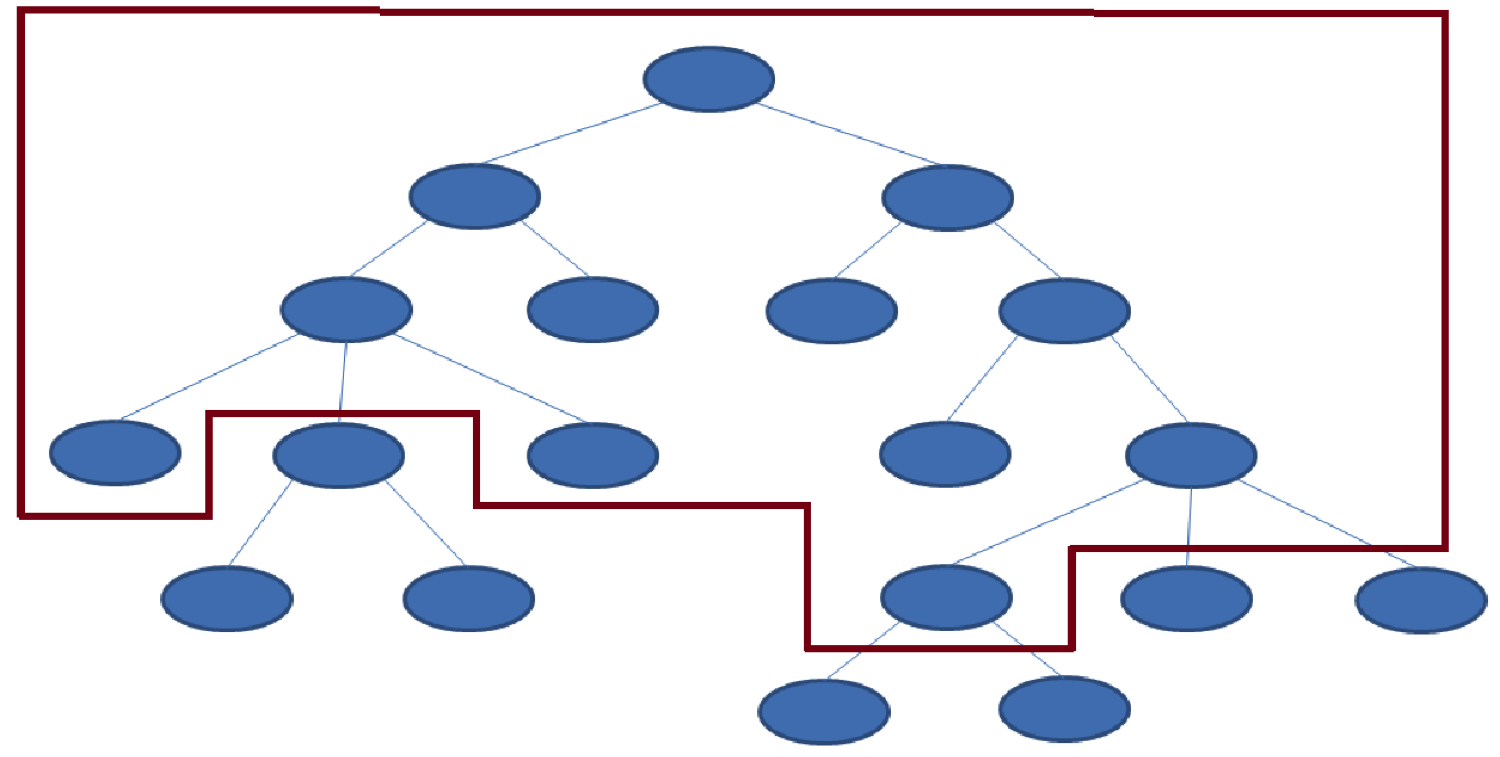
\includegraphics[scale=0.6]{arbolpoda}
  \caption{caption}

\end{figure}

%
